\documentclass[11pt]{article}
\usepackage{graphicx}
\usepackage{wrapfig}
\usepackage{geometry}
\geometry{
a4paper,
total={170mm,257mm},
left=20mm,
top=20mm,
}

\graphicspath{ {./images/} }

\title{Paper Template for COMP90049 Report}
\author{Zichun Zhu 784145\\
	\large zichunz@student.unimelb.edu.au}

\begin{document}
\maketitle
\section{Introduction}
This project is aimed to develop a multi-cliented dictionary. In more details, it should allow concurrent clients to search the meanings of a word, add a new word, and remove an exiting word. The project contains two part of system: the server and the client. The server have to be a multi-threaded that accepts multi-clients.

\section{Architecture}
\subsection{Server system}
The server is implemented as a thread-per-request architecture by Runnable. The reason mainly is the use of UDP protocol. The components in the server system for following: (See Figure \ref{fig:clientUML})
\begin{itemize}
\item Server: main function.
\item Utilities: contains all constants and utilities methods.
\item Dictionary: base dataset of dictionary, in format of json.
\item RequestObj: the construct of request object, including reading method.
\item ResponseObj: the construct of response object, including reading method.
\item Response: been implemented with Runnable. Once the socket received a message, one thread is created and each has one instance of response.
\item AckQueue: a hashmap that contains all acknologies from all clients. It is structured as $(clientIp + clientPort,\ Acknowledge\ Datagram)$. It also has synchronized $add$ and $remove$ method to be modified by threads.
\end{itemize}

\subsection{Client system}
The basic structure is sequential, but considering with the retransmission, one thread is created for this purpose. Concurrently, the main thread listens the responses from the server. When the response packet is received, the thread will be returned. The components in the server system for following: (See Figure \ref{fig:serverUML})
\begin{itemize}
\item Client: main function.
\item Utilities: contains all constants and utilities methods.
\item RequestObj: the construct of request object, including reading method.
\item ResponseObj: the construct of response object, including reading method.
\item GUI: using JFrame library to render.
\end{itemize}


\section{Implementation}

\subsection{UDP}
Comparing with TCP packets, UDP packets have shorter header. It led that UDP usually is a fast and efficient protocol. This benefit is significant in this project. Each request from the clients does not contain much data, and also the responses are about the length of words' definitions that are generally short. So this implementation is more similar to the DNS server, which can be performed highly efficiently.

On the other hand, the implementation with UDP also has some drawbacks. The largest issue it faced is dealing with the idempotent methods. It is important to note that UDP is an unreliable connection. Losing or unwanted modified packets could be happened frequently during the transmission. In this project there are three methods for the clients, and two of them, $add$ and $remove$, have to be idempotent. So how to make sure that these methods only run once, and regardless with network impact is the problem. The second issue is the limitation on sockets. In TCP, a socket is consisted of the address and port from the server, plus the address and port from the client. Thus it is unlikely that multiple processes take the same socket at the same time. While in UDP, because of the nature of connectionless, the socket is unable to initially bind with the destination. In a multi-thread program, the problem is correctly mapping different messages via the same socket to different threads.

To solve the first issue, there is an acknology message send if idempotent response returned. For example, $query$ is not an idempotent method. The system can be implemented exactly as the DNS server, which does not have any acknology send from client to the server. When the client does not receive the response in a certain period, it can simply send the same request again. However, such $add$ as idempotent methods do not allow. Thus once the server send a response, which in this case is "remove" method is whether success or fail, the client is required to send an acknowledge back to notice that response is received and no further duplicate $add$s are send. To dig deep into the algorithm, a recursive issue is obviously that neither server or client can stop sending acknology to the other side. The solution here unfortunately is perfect. When an idempotent request is send, the acknology will be stop after the client send an acknowledge for idempotent response. It may not be safe in some extreme situation. But it is the best algorithm I can think of, also it is similar to the solution by TCP. Moreover, retransmissions and checksum are applied as well to overcome the unpredicted network. In retransmission, RTT is set to a constant 200ms. Although it is better to be ajusted dynamicly like what TCP does, it is hard to get the underly level of netwoking. While TCP combined with IP is able to reach the condition of the network. 

For the second issue, it is important to collect all acknowledgements from client\footnote{The client does not receive any acknowledgement, rather than one response.}. AckQueue class is dedicated for collecting response, which has a key of $clientAdd+clientPort$. It is visible to all thread if they needed. Adding an ack of removing an ack are blocked to other modifier.

\subsection{JSON}
JSON standard for JavaScript Object Notation is one format created in earlier this century. In the era of web and HTTP birthing, JSON is used to transfer data with the lack of network bandwidth. It has the advantages that light weight structure and human readable style. And this implement can totally take the benefit over it. A lightweight structure means the short amount of data, which in some stage could reduce the risk of data missing or changing during the transmission. Java also has the native supported library for creating and parsing JSON formatted data.

\begin{figure}
	\centering
	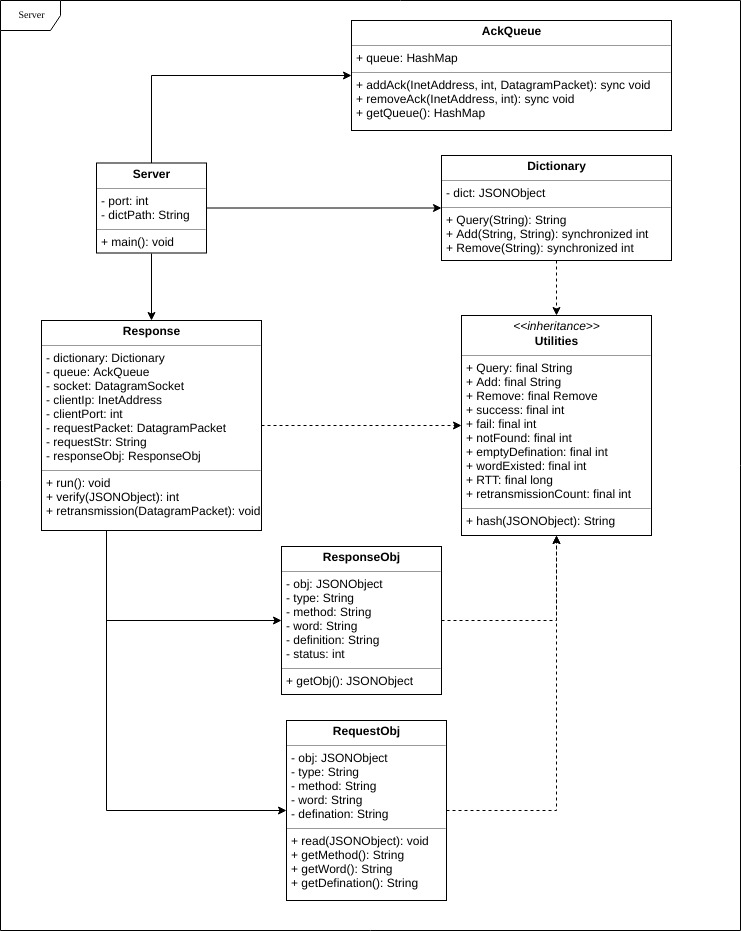
\includegraphics[width=\textwidth]{DS_Server}
	\caption{UML graph of Server system.}
	\label{fig:serverUML}
\end{figure}	

\begin{figure}
	\centering
	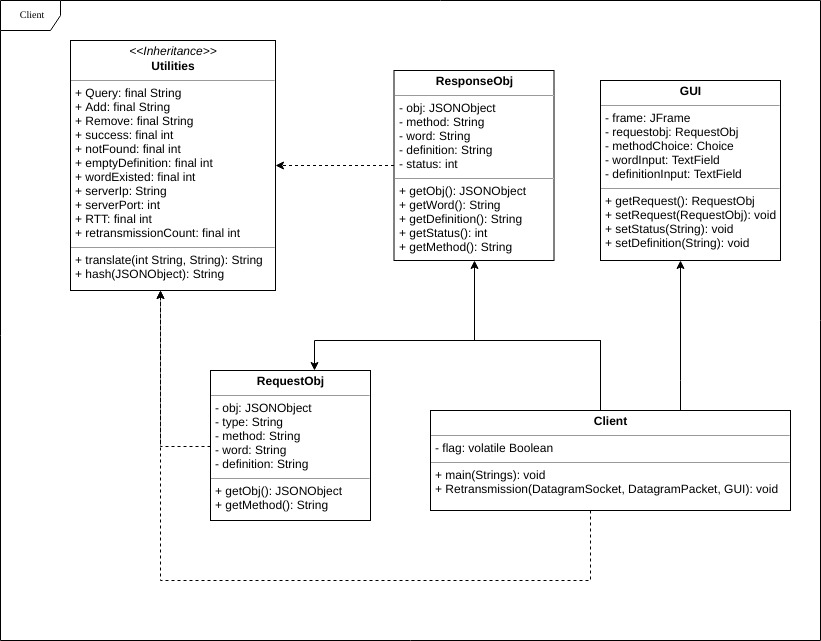
\includegraphics[width=\textwidth]{DS_Client}
	\caption{UML graph of Client system.}
	\label{fig:clientUML}
\end{figure}

\section{Conclusions}
This report introduced an implementation for a dictionary server and the recospond client. And also it discusses the features of this implementation.

\end{document}